% Repository:  https://github.com/chiehrosswang/TRB_LaTeX_tex
%
% Transportation Research Board conference paper template
% version 4.0 Lite (updates made to be compatible in Overleaf and ShareLaTeX)
%
%
% When numbered option is activated, lines are numbered.
\documentclass[numbered]{trbunofficial}
\usepackage{graphicx}
\usepackage{booktabs}

\newread\somefile
\usepackage{xparse}
\usepackage{natbib}
\bibliographystyle{unsrtnat}
\setcitestyle{round}
% \usepackage[colorlinks=true,linkcolor=blue,citecolor=blue]{hyperref}
% For TRB version hide links
\usepackage[hidelinks]{hyperref}

% Put here what will go to headers as author
\AuthorHeaders{Reynolds and Currie}
\title{Leveraging GTFS data to calculate an open-source Transit Supply
Index}

% TODO: add macros for easier formatting of \author.
\author{%
    \textbf{James Reynolds}\\\textit{Corresponding Author}\\
  Research Fellow\\
  Public Transport Research Group, Institute of Transport Studies,
Department of Civil Engineering, Monash University, Victoria,
Australia\\
  \href{mailto:james.reynolds@monash.edu}{\nolinkurl{james.reynolds@monash.edu}}\\
  \hfill\break
    \textbf{Graham Currie}\\
  Professor\\
  Public Transport Research Group, Institute of Transport Studies,
Department of Civil Engineering, Monash University, Victoria,
Australia\\
  \href{mailto:graham.currie@monash.edu}{\nolinkurl{graham.currie@monash.edu}}\\
  \hfill\break
  }

% If necessary modify the number of words per table or figure default is set to
% 250 words per table (default defined in cls)


% If words are counted manually, put that number here. This does not include
% figures and tables. This can also be used to avoid problems with texcount
% program i.e. if one does not have it installed.
\TotalWords{684}


% tightlist command for lists without linebreak
\providecommand{\tightlist}{%
  \setlength{\itemsep}{0pt}\setlength{\parskip}{0pt}}




\begin{document}
\maketitle


\section{Abstract}
TBC.
\hfill\break%
\hfill\break%
\noindent\textit{Keywords}:  Transit, Public
transport, GTFS, Benchmarking,  
\newpage

\hypertarget{introduction}{%
\section{Introduction}\label{introduction}}

Transit service level indicators include those in the Transit Capacity
and Quality of Service Manual (TCQSM) \citep{TCQSM:2013}, the Transit
Score metric and many more. Practitioners, researchers and advocates
seeking to use such metrics may face two inter-related challenges:
firstly, there is the problem of calculating the metrics themselves for
a specific location; secondly, is the challenge of explaining the
metrics, their meaning and importance those who are not specialists in
transit, such as politicians, other decision-makers or the general
public.

The TCQSM specifies Levels of Service (LOS) between A and F across a
range of factors including service span, frequency, speed, and the
proportion of population serviced. Previous research by
\citet{Wong:2013aa} overcame some challenges of using the TCQSM, by
using Python, PostgreSQL and R software and GTFS feeds as input to
automate the calculation of daily average headways, route length and
stop numbers. This indicators, however, are route based and so do not
include any consideration of geographic or population coverage. Further
metrics addressing these topics and much detail about their calculation
and meaning are included in the TCQSM, such as the Service Coverage Area
(pp.~5-8 to 5-21). However, these appear highly detailed, may required
bespoke GIS or other analysis, and it might be challenging to explain
these measures (beyond the fact at A is good and F is bad) to
non-technical decision-makers, stakeholders or others who might be
involved. Transit Score provides a similarly easily understood rating
scale, scoring locations out of 100 \citep{WalkScore:2023tg}. However,
the algorithm is patented and effectively a black box, meaning that it
is not possible to calculate scores independently to understand how the
metric might change with cahnges to the transit system or surrounding
environment.

The Supply Index developed by \citet{currie2007identifying} may provide
a metric that is relatively easy to calculate, open (rather than a black
box), and relatively simple for a non-technical audience to understand,
engage with and use. This Index is based on calculating the number of
transit arrivals at stops within an area of interest, with an adjustment
made for the amount of the area of interest that is within a typical
walk access distance of each stop. However, it does not appear to have
been widely used, perhaps in part because it still required an analyst
to obtain sources of timetable and geographic data. Since the
publication of \citet{currie2007identifying} such data has become much
easier to obtain with more than 10,000 agencies now providing timetable
and network data using the General Transit Feed Specification (GTFS)
format \citep{GTFS}. A gap, however, is that there is not yet a method
for calculating the \citet{currie2007identifying} Supply Index directly
from GTFS data.

This paper reports the development of R code to calculate the Supply
Index of \citet{currie2007identifying} directly from GTFS data. The code
is developed using data from a single case: the GTFS for Victoria in
Australia, which includes Greater Melbourne. Cross-case comparison to
Toronto, Canada, and Washington DC, USA, is also undertaken to test the
results and gain understanding of how the Supply Index might be useful
for practitioners, researchers and advocates. The motivation for this
research is to better understand how GTFS data might be used to produce
benchmarking metrics that can be calculated using open-source code, that
can be used to access proposed network changes and which may be
relatively easy for non-technical specialists to understand.

\hypertarget{research-context}{%
\section{Research context}\label{research-context}}

Even a brief search shows that there is a very large number of metrics
available for benchmarking transit services, for example: the Transit
Cooperative Research Program (TCRP) Report 88 provides an extensive
guidebook on developing a performance-measurement system
\citep{Ryus:2003aa}; online databases are provided by the Florida
Transit Information System (FTIS)
\citep{Florida-Transit-Information-System:2018aa} and the International
Association of Public Transport (UITP) \citep{UITP:2015aa} have online
databases, while the Transport Strategy Centre of Imperial College
London runs extensive annual benchmarking programmes across over 100
transit provides around the world
\citep{Imperial-College-London:2023aa}. The Fielding Triangle
\citep{FieldingGordonJ1987Mpts} provides a framework for understanding
how such metrics combine service inputs, service outputs and service
consumption to describe cost efficiency, cost effectiveness or service
effectiveness measures. At a larger scale, \citet{Litman:2003ab} and
\citet{Litman:2016aa} discuss some of the traffic, mobility,
accessibility, social equity, strategic planning and other rational
decision-making frames that might underlie such transit metrics, while
\citet{Reynolds:2017ah} extends this into models of how
institutionalism, incrementalism and other public policy models might
apply to decision-making processes. Further examples are provided by
\citet{GuzmanLuisA.2017Aeit}, who develop a measure of accessibility in
the context of policy development and social equity for Latin American
Bus Rapid Transit (BRT) based networks, and the street space allocation
metrics based around 10 ethical principles from
\citet{Creutzig2020streetspaceallocation}.

However, many of these metrics are difficult to calculate, complex to
explain or understand, and likely not well suited to communication with
those who are not transit planners or engineers, or otherwise technical
specialists. However, where pre-calculated metrics are immediately
available it may not be possible for generate metrics for proposed
system changes or know exactly how scores are calculated. The TCQSM and
Transit Score may provide contrasting examples: with respect to the
first challenge, TCQSM metrics may require large amounts of network,
service, population and other data to be assembled before the indicators
can be calculated; whereas Transit Scores are readily available on the
\citet{WalkScore:2023tg} website for locations with a published GTFS
feed (eliminating the need for any calculations). With respect to the
second challenge, the meaning of the Transit Score appears easy to
explain (the closer to 100, the better), but as the score is calculated
by a patented algorithm (effectively a black-box) it may not be easy to
understand or explain the connection between real-world conditions and
the score, or what might need to be done to improve the score and
service levels. Nor does it appear to be possible for Transit Scores to
be generated for proposed changes to networks. The TCQSM, in contrast is
open-source, in that \citet{TCQSM:2013} provide a manual describing all
the metrics and how to calculate them. However, the calculations
themselves appear to be complex, which may be a barrier to use by
practitioners, researchers, advocates or others who are not transit
scheduling specialists. While \citet{Wong:2013aa} provides open-source
code (\url{https://github.com/jcwong86/GTFS_Explore_Tool}) this is 11
years old and does not appear to be currently maintained. Future
research may involve reviewing this code and using it to analyse modern
GTFS feeds. However, in this paper the aim is more modest, in that the
objective is to develop code to calculate the simpler Suppy Index metric
from \citet{currie2007identifying}.

\hypertarget{the-suppy-index}{%
\subsection{The Suppy Index}\label{the-suppy-index}}

The Supply Index is shown in Equation \ref{eq:supply_index}. Minor
adjustments have been made to generalise the equation, as
\citet{currie2007identifying} focused on the context of Melbourne's
Census Collection Districts (CCD) and calculations based on a week of
transit service. \begin{equation}
\label{eq:supply_index}
  SI_{area, time} = \sum{\frac{Area_{Bn}}{Area_{area}}*SL_{n, time}}
\end{equation}

\(SI_{area, time}\) is the Supply Index for the area of interest and a
given period of time. \(Area_{Bn}\) is the buffer area for each stop (n)
within the area of interest. In \citet{currie2007identifying} this was
based on a radius of 400 metres for bus and tram stops, and 800 metres
for railway stations. \(Area_area\) is the area of the area of interest,
and \(SL_{n,time}\) is the number of transit arrivals for each stop for
a given time period.

An advantage of the Supply Index is that it is a relatively simple
number to calculate, understand and explain. It describes the number of
transit arrivals at stops within an area of interest and time frame,
multiplied by a factor accounting for the proportion of the area of
interest that is within typical walking distance of each stop. Hence,
more services, more stops and higher frequencies would all result in an
increase in Supply Index score. The Supply Index, however, does not
incorporate further aspects, such as service span, off-peak share of
service or service speed. However, including such metrics may increase
the complexity of calculating and describing the index to non-transit
specialists. Such simplicity is helped by the way that the Index is
additive, in that SI\textasciitilde area, time\textasciitilde{} scores
can be aggregated to calculate an overall score across multiple time
periods or for a region encompassing multiple areas of interest.

\citet{currie2007identifying} calculated the SI\textasciitilde area,
time\textasciitilde{} for various CCDs in Melbourne using a timetable
database provided by the Victorian Public Transport Authority (PTA).
This predated the widespread availability of GTFS data, which provides a
standardised format for timetable data that is produced by many transit
systems. GTFS is an open, text-based format that was developed
originally to allow transit information to be included in the Google
Maps navigation platform \citep{GTFS}. A question, therefore, is how to
calculate the SI using GTFS data so that SI\textsubscript{areas} can be
calculated and compared for any area of interest where transit service
information is available in the GFTS format.

\hypertarget{methodology}{%
\section{Methodology}\label{methodology}}

This study adopts a case research approach by developing code to
calculate Supply Indexes for Melbourne (Australia), Toronto (Canada) and
Washington D.C. (USA). The case research approach serves two purposes:
firstly the selected cases where used to develop, test and verify the
functionality of the code produced in this study. Secondly, aspects of
the the selected cases were explored;, such as the impact of forthcoming
upgrades and issues of level-boarding access (i.e.~non-step suitable for
wheelchair, pram, mobility-aid etc.) to the Supply Index scores.

\hypertarget{code-development}{%
\subsection{Code development}\label{code-development}}

Various analysis tools are available that make us of GTFS data,
including the tidytransit package \citep{tidytransit2023} for the R
statistical programming language \citep{R-base}.
\citet{tidytransit_departure_timetable} provides code to calculate a
departure timetable from a GTFS feed, and this was adapted to calculate
arrivals at a stop and the SL\textsubscript{Bn} term.

The gtfstools R package \citep{R-gtfstools} was used to split input GTFS
feeds by mode to facilitate the buffer zone calculation. Buffer zones of
400 metres for bus and Light Rail Transit (LRT) services and 800 metres
for heavy rail, as per \citet{currie2007identifying}. There is an
extended mode definition that includes modes beyond the 10 in the GTFS
standard \citep{filter_GTFS_by_mode}, but these are not dealt with by
the gtfstools package. Further research may seek to extend this such
that other modes can be included, but for the purposes of this study the
buffer zone was set at 400 metres for cable trams, aerial lifts such a
gondalas and trolleybuses, and at 800 metres for ferries, funiculars and
monorails.

Where transit stops are located close to boundaries their catchment
areas may fall into multiple areas of interest. The sp package from
\citep[\citet{applied_spatial_data_analysis_with_R}]{spatial_data_in_R}
provides tools for manipulating geographic data and shape files in R.
This is used to calculate the proportion of each stop's catchment area
that falls into each geographical area of interest. GTFS files define
stop locations based on latitude and longitude
\citep{GTFS_schedule_reference}, whereas the Area\textsubscript{Bn}
calculation needs to be provided in the same units as the
Area\textsubscript{area} variable. This therefore necessitates the use
of a geographic transform so that calculations can be undertaken in
metres.

The SI\textsubscript{area} was calculated on a mode-by-mode and
stop-by-stop basis, by first determining the amount of the catchment
area (Area\textsubscript{Bn}) that falls into each geographical area of
interest for the stop in question. This is combined with the area for
each geographical area of interest (Area\textsubscript{area}) and the
number of stop arrivals within the (SL\textsubscript{Bn}) to calculate
the contribution to the index scores made by just that single stop for
every area of interest (the SI\textasciitilde area, time, mode,
n\textasciitilde); these are then added to a cumulative total field for
each area of interest; and the calculations are repeated until all stops
and modes in the GTFS file have been included.

\hypertarget{case-research-approach}{%
\subsection{Case research approach}\label{case-research-approach}}

These three cases were selected as they are familiar to the researchers,
and as there is likely to be enough variety in how the GTFS feeds,
potential areas of interest and other aspects are set up such that the
developed code will likely be generalis-able to other places.
Additionally, the case selection continues the long-standing practice of
comparing Melbourne and Toronto, as well as grounding one of the three
cases in the context of the transit system where the Transportation
Research Board Annual Meeting is located (which is likely to be familiar
to many readers).

\hypertarget{melbourne-victoria-australia}{%
\subsubsection{Melbourne, Victoria,
Australia}\label{melbourne-victoria-australia}}

Greater Melbourne is a geographic area that is similar to that of the
metropolitan areas of Paris or London, but with only around 5 million
people has about one-third of the population. It consists of a inner
Central Business District (CBD) with appartments, commercial skyscrapers
and extensive sporting facilities nearby; surrounded by low-density,
predominately single-family-housing-dominated, inner, middle and outer
suburbs.There are predominately radial train and tram networks, but for
most of the suburban areas the reality is that transit is provided by
circuitious bus routes that are mostly used by those who cannot
otherwise drive. An extensive freeway (and tollway) network provides
connections across the Greater Melbourne area, further around Port
Phillip Bay to Geelong (south-west) and the Mornington Penninsula
(south-east) as well as to regional centres elsewhere in Victoria. There
is a state-wide regional train and bus network, which also provides
connections into South Australia, New South Wales and the Australian
Capital Territory (Canberra) and local bus services in many regional
towns and cities. However, accessibility to most of the city and state
tends to be car-dominated, with transit mode share only accounting for
XX\% across Greater Melbourne and YY\% across Victoria. The
journey-to-work transit mode shares, however, are ZZ\% across Greater
Melbourne and PP\% for travel into the CBD, which is reflective of the
monocentric nature of the railway network, which focuses on Southern
Cross Station (Spencer Street) for regional services and on a
five-station City Loop (Southern Cross, Flinders Street, Parliament,
Melbourne Central and Flagstaff) the helps to distribute commuters to
workplaces across the CBD.

Melbourne's GTFS feed is published by Public Transport Victoria (PTV).
There are over 400 historical releases of the available on the
transitfeeds.com website, with the first dating from March 2015
\citep{transitfeeds_victoria:2023aa}. The Australian census is
undertaken in early August every 5 years, with the last two being in
2016 and 2021. GTFS feeds were therefore selected for the first week of
August of each year for the purposes of this test analysis, so that the
date of measurement of the Supply Index matches the census dates.

Minor corrections were made to the GTFS files to remove duplicate
stop\_ids. These involved minor discrepancies in either the stop name,
latitude or longitude. The Australian Bureau of Statistics (ABS)
provides a range of shape files and other resources, and this study made
use of the absmapsdata R package \citep{R-absmapsdata} to access the
2021 Local Government Area (LGA) boundaries for the Greater Melbourne
area. The EPSG:28355 transform \citep{EPSG_28355} was used to shift
longitude and latitude into metres, as per the Geocentric Datum of
Australia 1994 (GDA95 / MGA zone 55) coordinates.

\hypertarget{toronto-ontario-canada}{%
\subsubsection{Toronto, Ontario, Canada}\label{toronto-ontario-canada}}

\hypertarget{washington-dc-usa}{%
\subsubsection{Washington DC, USA}\label{washington-dc-usa}}

\hypertarget{results}{%
\section{Results}\label{results}}

The code is available at
\url{https://github.com/James-Reynolds/Transit_Supply_Index_GTFS} as an
Rmarkdown file (used to typeset this paper). The following subsections
discuss the results of cases studies used to develop and test the code.

\hypertarget{victoria-australia}{%
\subsection{Victoria, Australia}\label{victoria-australia}}

\hypertarget{transit-supply-index}{%
\subsubsection{Transit Supply Index}\label{transit-supply-index}}

\begin{figure}
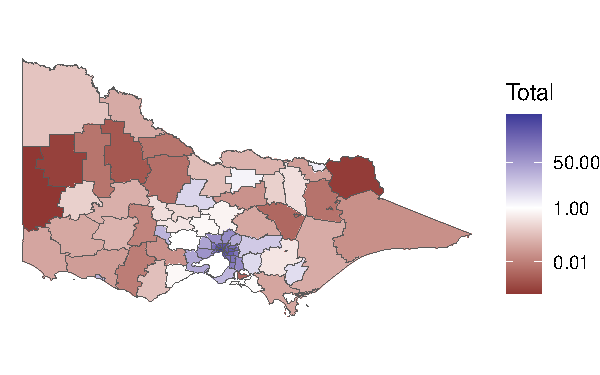
\includegraphics[width=0.5\linewidth]{Reynolds_Currie_2024_transit_supply_index_GTFS_files/figure-latex/Victoria_SI_2021-1} 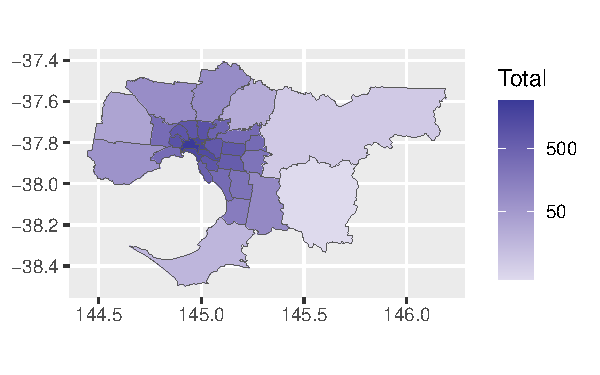
\includegraphics[width=0.5\linewidth]{Reynolds_Currie_2024_transit_supply_index_GTFS_files/figure-latex/Victoria_SI_2021-2} \caption{SI for 2021 census day (August 10th) by LGA}\label{fig:Victoria_SI_2021}
\end{figure}

\begin{figure}
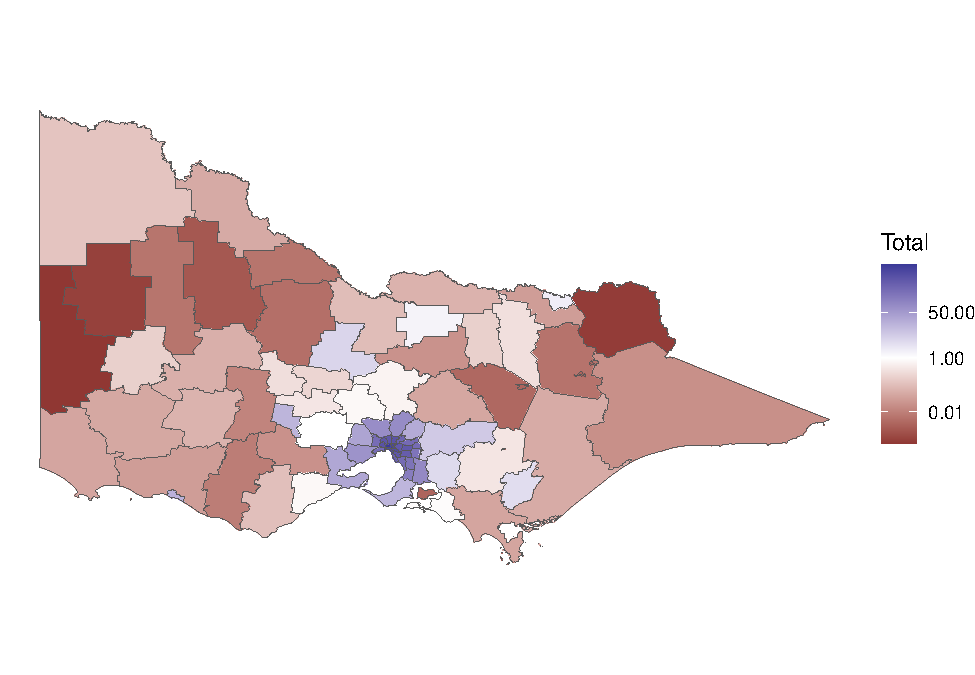
\includegraphics[width=0.5\linewidth]{Reynolds_Currie_2024_transit_supply_index_GTFS_files/figure-latex/Victoria_SI_2016-1} 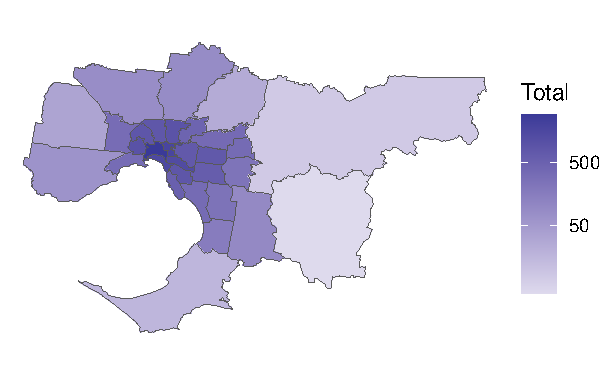
\includegraphics[width=0.5\linewidth]{Reynolds_Currie_2024_transit_supply_index_GTFS_files/figure-latex/Victoria_SI_2016-2} \caption{SI for 2016 census day (August 9th) by LGA}\label{fig:Victoria_SI_2016}
\end{figure}

\hypertarget{transit-needs}{%
\subsubsection{Transit needs}\label{transit-needs}}

\hypertarget{level-boarding-accessibility}{%
\subsubsection{Level-boarding
accessibility}\label{level-boarding-accessibility}}

\hypertarget{the-metro-tunnel---adding-services}{%
\subsubsection{The metro tunnel - adding
services}\label{the-metro-tunnel---adding-services}}

\hypertarget{the-suburban-rail-loop}{%
\subsubsection{The suburban rail loop}\label{the-suburban-rail-loop}}

\hypertarget{toronto}{%
\subsection{Toronto}\label{toronto}}

\hypertarget{level-boarding-accessibility-1}{%
\subsubsection{Level-boarding
accessibility}\label{level-boarding-accessibility-1}}

\hypertarget{transit-city-what-might-have-been}{%
\subsubsection{Transit City: what might have
been}\label{transit-city-what-might-have-been}}

\hypertarget{viva-transit-what-was-achieved}{%
\subsubsection{Viva transit: what was
achieved}\label{viva-transit-what-was-achieved}}

\hypertarget{downtown-relief-lines}{%
\subsubsection{Downtown relief lines}\label{downtown-relief-lines}}

Many proposals - look at a few of them?

\hypertarget{washington-dc}{%
\subsection{Washington DC}\label{washington-dc}}

\hypertarget{level-boarding-accessibility-2}{%
\subsubsection{Level-boarding
accessibility}\label{level-boarding-accessibility-2}}

\hypertarget{cross-case-comparison}{%
\subsection{Cross-case comparison}\label{cross-case-comparison}}

\hypertarget{discussion}{%
\section{Discussion}\label{discussion}}

\hypertarget{conclusions}{%
\section{Conclusions}\label{conclusions}}

\hypertarget{author-contribution-statement}{%
\section{Author Contribution
Statement}\label{author-contribution-statement}}

The authors confirm contribution to the paper as follows: study
conception and design: A. Anonymous, D. Zoolander; data collection: B.
Security; analysis and interpretation of results: A. Anonymous, B.
Security; draft manuscript preparation: A. Anonymous. All authors
reviewed the results and approved the final version of the manuscript.

\hypertarget{acknowledgements}{%
\section{Acknowledgements}\label{acknowledgements}}

This document was prepared using the \texttt{rticles} template, created
by Gregory Macfarlane, which is based on the \LaTeX originally posted by
David Pritchard in 2009 and updated it in 2011, soon after TRB began
allowing PDF submissions. Gregory Macfarlane and Ross Wang made
adjustments to the template, and Ross Wang now maintains the
\LaTeX template at \url{https://github.com/chiehrosswang/TRB_LaTeX_tex}.
Gregory Macfarlane created the \texttt{rticles} template in 2021.

\newpage
\renewcommand\refname{References}
\bibliography{packages.bib,References.bib}


\end{document}
